\documentclass[a4paper]{article}
\usepackage[utf8x]{inputenc}
\usepackage[T1]{fontenc}
\usepackage{graphicx}
\usepackage{xcolor}
\usepackage{wallpaper}
\usepackage[french]{babel}
\usepackage{array}
\usepackage[top=2cm,bottom=2cm,left=2cm,right=2cm]{geometry}

\begin{document}

%--------------
% page de garde
%--------------
\ThisLRCornerWallPaper{1}{rules.png}
\color{white}
\begin{titlepage}
	\begin{center}
		\Large{Année universitaire 2016-2017}\\
		\Large{Université de Caen Basse-Normandie}\\[1cm]		
		\huge Livre de règles pour Wargame des Faquins\\[0.5cm]
		\vspace{1cm}
		CANUET Maxime, CORBET Thorvald, JOLIVEL Valentin, L'HOMME Florentin\\
		\normalsize{\textit{ ~ L2 Informatique}}
		\vspace{2cm}
	\end{center}
\end{titlepage}

\newpage

%-----------
% sommaire
%-----------
\color{black}
\ThisLRCornerWallPaper{1}{img/fond.png}
	\tableofcontents
\newpage

%------------------------
% début du compte rendu
%------------------------

\section{règle générale}

\ThisLRCornerWallPaper{1}{img/fond.png}

	\quad Pour pouvoir jouer au Wargame il vous faudra respecter les règles qui suivent, ces dernières seront pour la plupart expliquées plus en détail par la suite.

	\subsection{Principe du jeu}

	\quad Le principe du jeu est de faire combattre deux armées qui auront été préalablement déterminées par les joueurs (\textit{cf: chapitre sur les armées}). Le mode de jeu est de type annihilation, autrement dit la victoire sera donnée à l'armée qui restera en vie, le joueur qui n'a plus d'unité en vie perd la partie. Le jeu se joue en tour par tour sans limite de temps. Un tour se divise en deux phases de jeu. La première phase est la phase de déplacement, la deuxième est la phase d'action (\textit{cf: chapitre sur les phases de jeu}). Une fois qu'un joueur a effectué ses deux phases, c'est au tour du joueur suivant. Une fois que tous les joueurs ont joué leurs deux phases un nouveau tour commence, cette mécanique se poursuit du moment que l'un des deux joueurs possède encore au moins une unité. Il n'y a pas de limite de temps pour jouer son tour ni de limite de tours pour une partie.

	\subsection{Les statistiques des unités}
	
	\quad Chaque unité qui compose votre armée possède 9 statistiques différentes. Chaque statistique joue un rôle propre sur l'attaque ou la défense de votre unité.
	
	\begin{description}
	
		\item[Point de vie (PV): ]Les points de vie représentent les dégâts que peut encaisser l'unité avant de mourir.
		\item[Armure (DEF): ]Les points d'armure représentent le pourcentage de réduction de dégât(\textit{PA=10, les dégâts qu'elle subit sont réduits de 10\%}).
		\item[Attaque (ATQ): ]Les points d'attaque représentent les dégâts que peut infliger votre unité si la cible n'a pas d'armure.
		\item[Déplacement (MVT): ]Les points de déplacement représentent le nombre maximal de cases que votre unité peut parcourir.
		\item[Précision (PRE): ]La précision représente le pourcentage de chance que votre unité a de toucher l'unité que vous attaquez (\textit{PRE=50, votre unité a 50\% de chance de toucher lors d'une attaque}).
		\item[Portée: ]La portée représente la distance (\textit{en nombre de cases}) à laquelle vous pouvez attaquer, vous ne pouvez pas attaquer des unités au delà de ce nombre (\textit{si la valeur est 1 alors l'unité ne peut attaquer qu'au corps à corps}).
		\item[Taux d'esquive(ESC): ]Le taux d'esquive représente le pourcentage de chance de votre unité à esquiver une attaque réussie de l'unité adverse(\textit{ESC=10, vous avez 10\% de chance de ne prendre aucun dégât si l'ennemi réussi son attaque}).
		\item[Taux de critique(CRIT): ]Le taux de critique représente le pourcentage de chance que votre unité à de faire une attaque critique si vous avez réussi votre attaque. Si vous réussissez une attaque critique les dégâts sont augmentés de 1.5 fois leur valeur de base (\textit{sans prendre en compte l'armure}).
		\item[Prix: ]Le prix représente le coût en point d'une seule unité (\textit{cf: composer une armée}).
		
	\end{description}

\newpage
\section{Phases de jeu}
\ThisLRCornerWallPaper{1}{img/fond.png}

	\subsection{Phase de déplacement}

	\quad Durant cette phase vous pouvez bouger n'importe quelle unité de votre armée. Chaque unité peut se déplacer d'un nombre de cases précis, cette valeur vous est donnée par un tableau au début de la section concernant votre armée. Vous pouvez bouger vos unités dans la direction que vous voulez il suffit de tracer le chemin que l'unité doit emprunter avec votre souris.

	\hspace{.3cm}

	\quad Votre déplacement n'est pas valide si il finit en dehors de la carte, si il finit sur un obstacle infranchissable, si il finit sur une case avec une unité déjà présente dessus.

	\quad Votre unité peut librement passer au travers de troupes alliées cependant si, lors de son déplacement, votre troupe se trouve sur la case adjacente à une troupe ennemie ,alors votre troupe est forcée de s'arrêter et tous ses points de déplacement sont annulés.

	\quad Si votre troupe est en combat (\textit{si elle se trouve sur une case adjacente à une troupe ennemie}) alors elle ne peut pas se déplacer. Le combat doit se terminer (\textit{une unité doit mourir}) avant que l'une des deux unités ne puisse bouger.

	\begin{figure}[h]
		\center
		\includegraphics[scale=.6]{img/mvts.PNG}
		\caption{schéma de mouvement possible et impossible}
	\end{figure}

	\newpage
\subsection{Phase d'action}
\ThisLRCornerWallPaper{1}{img/fond.png}

	\quad Durant cette phase vous allez décider de l'action que vas effectuer votre unité. Vos pouvez attaquer si vous êtes à une distance suffisante pour le faire(\textit{cf tableau de l'armée case portée}), vous mettre en posture de défense ou ne rien faire.
	
	\subsection{Attaquer}

	\subsubsection{Celui qui attaque :}	
	
	\quad Si vous décidez d'attaquer, il faut que l'unité que vous désirez attaquer soit sur une case adjacente si il s'agit d'une attaque au corps à corps, ou à un nombre de case inférieur ou égale à votre portée si il s'agit d'une attaque à distance. Si vous êtes sur une case adjacente à une unité ennemie alors vous ne pouvez pas utiliser une attaque à distance.

	\quad \textbf{Etape 1: }	
	
	\quad Si vous validez la condition de distance alors vous pouvez attaquer. Un chiffre est choisi aléatoirement entre 0 et 100 compris, si ce chiffre est inférieur ou égal à votre précision, l'unité réussi son attaque, sinon elle rate son attaque et termine sa phase d'action. Si vous réussissez votre attaque, un deuxième chiffre entre 1 et 100 compris est choisi, si ce chiffre est inférieur ou égal à votre taux de critique, vous réalisez une attaque critique (\textit{1.25 fois vos dommages}).
	
	\quad \textbf{Etape 2: }
	
	\quad Si vous réussissez votre attaque, l'ennemi subit vos dommages moins sa réduction de dégât (\textit{sat armure}). Si ATQ=20 et PA(\textit{ennemi})=10, dégâts infligé = ATQ-(ATQ*(PA/100)) soit 18 points de dégâts, l'ennemi perd 18 points de vie.
	
	\subsubsection{Celui qui se fait attaquer :}
	
	\quad Si vous vous faites attaquer, votre unité a une chance d'esquiver et de contre-attaquer. L'esquive et la contre attaque ne sont possibles que si l'unité est au corps à corps.
	
	\quad \textbf{Étape 1(\textit{Esquiver}):}
	
	\quad Si l'unité ennemie a réussi son attaque (\textit{critique ou non}) viens votre phase d'esquive, un nombre est choisi aléatoirement entre 0 et 100 compris, si ce nombre est inférieur ou égale à votre esquive, vous esquivez le coup de l'adversaire. Ce qui a pour effet d'annuler l'attaque de l'adversaire. Si vous ratez votre esquive vous subissez l'attaque normalement(\textit{avec l'effet de critique si c'est une attaque critique})Sauf si vous vous êtes mis au préalable en posture de défense, dans ce cas allez au chapitre \underline{se défendre}.
	
	\quad \textbf{Étape 2 (\textit{Contre-attaquer}): }
	
	\quad Si vous avez réussi votre esquive, on choisi un deuxième numéros entre 0 et 100 compris, si ce numéros est inférieur ou égale à la précision de votre unité, vous pouvez contre-attaquer. L'ennemi ne peut pas esquiver une contre-attaque. Si vous ratez votre contre-attaque, il ne se passe rien.
	
	\quad Si vous réussissez votre contre-attaque l'ennemi subit la moitié de vos dégâts moins son armure. ATQ=20, PA(\textit{ennemi})=10 dommages= ATQ/2-(ATQ/2*(PA/100)) soit 6 points de dégât, l'ennemi perd 6 points de vie.

	\subsection{Se défendre: }
	
	\quad Si vous décidez de passer en posture de défense, l'armure de l'unité que vous avez sélectionné se voit augmentée de 20\%. Si DEF=20, alors 20*1.2=21, durant le tour de l'adversaire, votre unité aura 21 points d'armure au lieu de 20.

\section{Composer une armée}

	\quad Avant de jouer il vous faudra tout d'abord composer votre armée. Les joueurs sont libres de composer leur armée avec les unités qu'ils souhaitent, du moment que les règles suivantes sont respectées.
	\begin{itemize}
		\item Le générale de l'armée choisi doit être présent, ses points ne sont pas comptés dans le décompte total des points de l'armée.
		\item Le joueur ne peut pas mélanger les unités de différentes armées, il ne peut prendre qu'un seul général et seulement les unités qui sont dans la même armée que le général.
		\item Au début de la partie un nombre maximal de points est donné, l'armée construite par le joueur ne peut pas dépasser ce nombre de points, le nombre de point d'une armée est obtenu en additionnant la statistique prix de chaque unité de l'armée.
	\end{itemize}

	\newpage
\section{Les unités}
\ThisLRCornerWallPaper{1}{img/fond.png}

	\quad Chaque armée possède des unités qui lui sont propres, avec des statistiques et des prix différents, cette partie vous décri les unités de chaque armée.

\subsection{Les généraux}

	\quad\underline{\textbf{La Reine du chaos: }}
	
	\quad La Reine du chaos est une divinité pour les démons et une infamie pour tous les autres. L'énergie démoniaque qui coule en elle lui permet d'être une unité efficace à la fois à distance mais aussi au combat rapproché. Elle est le général ayant le plus grand pourcentage d'esquive et de chance de coup critiques. Sont pouvoir lors du combat est de donner à toutes ses unités une capacité de régénération durant un tours. Cette capacité se traduit par le fait que ces unités ont 50\% de chance de récupérer 20\% de leurs dégâts d'attaque (\textit{après réduction d'armure}) en temps que point de vie. \\
	
	 \quad\underline{\textbf{Général des Elfes:} }
    
 	\quad Le général des armées Elfes est l'unité la plus aguerrie dans leur domaine de prédilection : l'attaque à distance. Accompagné d'un fidèle destrier, le général a la possibilité de se déplacer rapidement pour venir en aide à ses troupes. Grâce à sa grande précision, acquise dans de nombreux exercices, il ne ratera jamais une cible à portée de main, quant aux cibles plus éloignées, il reste le meilleur tireur que le monde n'ait jamais connu. Conscient de la nécessité de sacrifice, le général ordonna à ses troupes, dès le début de la Guerre, de préférer l'attaque au déplacement si cela peut s'avérer devenir un avantage.\\
 	
 	\quad\underline{\textbf{Chef de guerre Ork: }}
	
	\quad Il arrive qu'un Ork tape plus fort que les autres, soit plus gros et plus fourbe. Ont leur attribue alors naturellement le commandement d'une troupe ( du moins jusqu'à ce qu'un Ork plus gros et plus fort vienne prendre sa place ). On appelle ces Orks des chefs de guerre.\\
	
	\quad\underline{\textbf{Le Jarl:} }
	
	\quad Un membre de la royauté Naines sur un bouc. Lourdement armé, une armure épaisse, un déplacement amélioré par le bouc de guerre sans oublier la charge de ce fidèle destrier. Une petite masse montée, pour la gloire des peuples Nains!!
	
	\quad\underline{\textbf{Le général de l'armée des humains.}}
	
	\quad Le général fait preuve d'une grande expérience de combat ce qui fait de lui l'unité la plus puissante de son armée. Accompagné de son fidèle destrier, il parcourt les champs de bataille allant de victoire en victoire au nom de son roi et de son peuple.
	
	\newpage
\subsection{Humains}

	\ThisLRCornerWallPaper{1}{img/races/humain.png}

	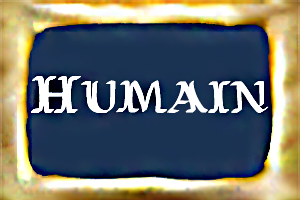
\includegraphics[scale=0.4]{img/tableau_armee/humain.PNG}
	
	\subsubsection{Les enrôlés: }
	
	\quad Unité faible et souvent alcoolisée de l'armée des humains, ces unités sont sur le terrain contre leur grès. 
	
	\subsubsection{Les épéistes: }
	
	\quad Les épéistes sont le cœur de l'armée humaine ils sont polyvalents et en grand nombre. 
	
	\subsubsection{Les chevaliers: }
	
	\quad Les chevaliers sont la fierté de l'armée humaine, leur forte défense ainsi que leur puissance de frappe font d'eux l'unité d'élite de cette armée.
	
	\subsubsection{L'archer: }
	
	\quad L'archer, malgré son manque évident de défense, se repose sur son esquive modérée ainsi que sa capacité à attaquer à distance.
	
	\subsubsection{L'arbalétrier: }
	
	\quad Comme les archers, leur défense est faible, cependant ils restent plus résistants que l'archer. Son arbalète lui permet de tirer plus loin ainsi que de façon plus précise.
	
	\subsubsection{Les cavaliers: }
	
	\quad Unités de choc, la cavalerie est la première à arriver au combat. Cependant il leur faudra faire attention aux unités équipées de lances qui pourront leur faire énormément de dégâts.

	\newpage
\subsection{Orks}

	\ThisLRCornerWallPaper{1}{img/races/ork.png}

	
\includegraphics[scale=.4]{img/tableau_armee/orks.PNG}
	
	\subsubsection{Gobelin}
	
	\quad Petit et faible, le gobelin est le fidèle serviteur des orks. Parfait pour courir jusqu'aux lignes ennemis et infliger de petits coups très frustrant, le gobelin reste une unité très fragile qui sera éliminée d'un revers de main.

	\subsubsection{Ork}
	
	\quad L'ork est la troupe de base de l'armée à la peau verte. Son manque de précision et son armure en peau de mouton sont compensées par une robustesse remarquable et une violence dont peu de races sont capables.

	\subsubsection{Piquier}
	
	\quad Le piquier est semblable au simple Ork, cependant, à cause de sa carrure plus frêle, ses dégâts et ses points de vie sont moins importants. Mais gare au cavalier qui se risquerait à négliger la lance de ce dernier...

	\subsubsection{Ork noir}
	
	\quad Plus gros, plus fort et moins intelligent que ses semblables Orks, l'Ork Noir possède une peau épaisse et une arme plus grosse, cela lui procure un potentiel à la fois offensif et défensif plus important.

	\subsubsection{Archer}
	
	\quad L'Archer Ork est une classe contre nature. Délaissant le plaisir de la mêlée au profit d'un arc de mauvaise qualité, il déchaîne sur l'ennemi une pluie de flèches incertaines.

	\subsubsection{Troll}
	
	\quad Très grand, très fort et très idiot. Le Troll représente un idéal Ork, et nombreux sont ceux qui désirent en devenir un ( bien que cela leur soit impossible... ).

	\subsubsection{Cavalier Warg}

	\quad Si l'Ork commun est une repoussant pour la plupart, les Cavaliers Warg n'ont pas leur pareil dans ce domaine. Rapides et puissants, il est difficile d'esquiver les attaques du cavalier ET de sa monture.

	\newpage
\subsection{Elfes}

	\ThisLRCornerWallPaper{1}{img/races/elfe.png}

	\includegraphics[scale=.4]{img/tableau_armee/elfe.PNG}
	
	\subsubsection{Elfes de maison: }
	
	\quad Ces êtres, plus petits que les autres elfes, n'ont initialement qu'un but dans leur vie : Celui de servir une maison. Autrement dit, ils ont habituellement pour tâches de nettoyer les saletés, de préparer les repas et répondre à toutes autres exigences de leurs maîtres. La guerre faisant rage, ces petits elfes sans importance ont été appelés sur le front. Toujours au service de leurs maîtres, ces créatures sont prêtes à donner leur vie pour eux.
	
 	\subsubsection{Archers Elfes: }
 	
 	\quad Le peuple Elfe s'est, au fil du temps, particulièrement spécialisé dans l'art de la guerre à distance. Les Archers Elfes représentent donc la base de leur armée, avec un peu d'entrainement, tout Elfe normalement constitué peut compter occuper ce poste s'il souhaite s'engager dans l'armée.
 	
 	\subsubsection{Archers Longs: }
 	
 	\quad A force d’entraînements, certains Archers Elfe peuvent rêver atteindre ce grade. Plus performantes qu'à leur début, ces unités sont plus précises, tirent de plus loin et, grâce à leur arc amélioré, infligent d'avantage de dégâts. Néanmoins ce nouvel armement a pour conséquence de les ralentir légèrement dans leur avancée.
 	
 	\subsubsection{Elfes furtifs: }
 	
 	\quad Les Elfes ne sont pas seulement habile à distance, ils le sont aussi dans les déplacements furtifs. Les Elfes furtifs ont été entraînés très jeunes à se déplacer rapidement tout en se fondant dans le décor. Malheureusement, pour préserver leurs facultés de déplacement et de discrétion, ces Elfes ne sont munis que d'armes blanches provoquant relativement peu de dégâts. Néanmoins, ce faible armement leur permet aussi d'esquiver plus aisément les attaques ennemies.
 	
 	\subsubsection{Hauts Elfes: }
 	
 	\quad Bien que spécialisé au combat à distance, les Elfes ont dû entraîner plusieurs de leurs compagnons au combat rapproché. Rare à suivre ces entraînements, les engagés ont une haute place dans l'estime de leurs compagnons, d'où leur appellation "Haut Elfe". Ces derniers suivent donc des entraînements leurs permettant de tenir un front, lourdement équipés, ils peuvent recevoir de multiples coups et en affliger de plus durs à leurs ennemis.
 	
	\subsubsection{Mages Elfiques: }
	
 	\quad Le peuple Elfique est doté de magie, en effet, avec un peu d'entraînement, et d'enseignement des anciens, chacun d'eux peut éveiller les forces élémentaires qui sommeillent en lui. N'utilisant initialement pas ce domaine dans la guerre, les attaques des Mages Elfiques ne font pas trop de dégâts, en revanche leur précision est très grande ! Parfois, des réactions en chaine peuvent provoquer quelques dégâts critiques.
 	
 	\subsubsection{Golems: }
 	
 	\quad Ces créatures sont inelfiques, elles ne possèdent aucune d'intelligence et leur masse ne leur permet que peu de mouvements. Au début de la Guerre, les Anciens Mages Elfiques ont voulu se rendre utiles malgré leur vieil âge et leur mobilité réduite. Ils se sont alors rassemblés et ont unis chacune de leur spécialité en magies élémentaires. L'union de ces magies a permis dans un premier temps de former une masse compacte, prête à encaisser les coups ennemis, ensuite, les Anciens se sont rassemblés en cercle et ont commencé à mener des incantations incessantes pour animer ces masses d'éléments. Ainsi est le Golem: Une masse d'éléments créée et animée par les Anciens Mages Elfiques.

	\newpage
\subsection{Nains}

	\ThisLRCornerWallPaper{1}{img/races/nain.png}

	\includegraphics[scale=.4]{img/tableau_armee/nain.PNG}
		
	\subsubsection{Mineurs}

	\quad Le Mineur n'est pas un guerrier. Il est avant tout un fier travailleur qui vient proposer main forte à ses compères pour écraser les armées ennemies. Leurs attaques à la pioche ne font pas beaucoup de dégâts et ne portant pas d'armure ils ne possèdent pas une grande résistance.

	\subsubsection{Barbepierre}
	
	\quad Les Barbepierre sont des anciens guerriers Nains qui, forts de leurs expériences, se sont décidés à combattre jusqu'à leur mort. Comme les guerriers Nains, ils possèdent un nombre de point de vie relativement élevé et une bonne défense. Du fait de leurs connaissances du combat ils possèdent un taux de critique légèrement plus élevé que les Brisefer.

	\subsubsection{Sprinter}
	
	\quad Comme le dis le Maitre Nain Gimli:"Nous les Nains sommes des sprinter, redoutable sur les courtes distances!". Les Sprinters sont les unités qui se déplacent le plus rapidement chez les Nains. Rapide, efficace.

	\subsubsection{Brisefer}

	\quad C'est la troupe de choc Naine. Des soldats lents mais puissants! Les victoires des plus grandes batailles des Nains sont souvent permises par ces fiers guerriers. Un taux de critique respectable et une armure à toute épreuve.

	\subsubsection{Berzerk}
	
	\quad Les Berzerks sont des Nains entrés dans une transe de combat. A peine raisonnables, ils écoutent leur Jarl mais massacrent leurs ennemis avec tout ce qu'ils peuvent. Des gros points de vie, de la grosse armure et un gros Nain qui court vite, que demander de plus?

	\subsubsection{Branner}
	
	\quad A force de creuser, les Nains sont arrivé dans les tréfonds. Arrivé en ce lieu emplis de Magma, ils durent trouver un moyen de faire de l'espace. C'est ainsi que le Branner naquit. Un soldat transportant des sceaux de lave pour les lancer sur ses ennemis. Lent mais violent.

	\subsubsection{Ingenieur}
	
	\quad L'Ingénieur Nain peut être utilisé pour la bataille. En effet l'utilisation de la poudre peut permettre d'exploser quelques Orks malotrus qui se seraient dressés sur leurs chemin. Cette unité à distance Nains fais énormément de dégâts mais ne se déplace pas vite, la lave ça brule!! 

	\newpage
\subsection{Démons}

	\ThisLRCornerWallPaper{1}{img/races/demons.png}

	
\includegraphics[scale=.4]{img/tableau_armee/demons.PNG}
	
	\subsubsection{Rejetons: }
	
	\quad Les Rejetons sont les unités les plus faibles de l'armée des démons, cependant leur faible capacité de combat et de défense sont compensées par leur capacité de mouvement (\textit{qui est l'une des plus grande toutes les armées confondues}) ainsi que leur faible prix. Ces unités ne sont donc pas faites pour gagner leur combat, cependant elle peuvent gêner les déplacements de vos ennemis.
	
	\subsubsection{Les Soldats de la Reine: }
	
	\quad Les Soldats de la Reine sont des unités polyvalentes, leur déplacement et leurs caractéristiques ne sont pas exceptionnelles, cependant leur prix non plus, il constitueront le cœur de votre armée.
	
	\subsubsection{Lanciers déterrés: }
	
	\quad Ces unités sont très semblables aux Soldats, cependant ces dernières étant équipées de lance, elle bénéficient de gros avantages face à la cavalerie.
	
	\subsubsection{Les Gardes de la Reine: }
	
	\quad Ces unités sont la fierté de l'armée des démons. Leur puissance d'attaque ainsi que leur lourde défense font de ces unités les plus puissantes de cette armée. Cependant leurs déplacements réduits les empêchent d'arriver les premiers lors des combats rapprochés. Cependant leur titre en dit long sur leur rôle.
	
	\subsubsection{Cracheurs d'acide: }
	
	\quad Ces créatures répugnantes ont acquis la capacité de cracher de l'acide sur leurs ennemis. Les attaques de ces créatures feront de gros dégâts au sein des armées ennemies, leur condition de créature leur font bénéficier d'une bonne précision ainsi que d'un déplacement amélioré. Cependant il vous faudra faire attention car, malgré leur aspect répugnant, ils n'en restent pas moins des démons avec une faible armure.
	
	\subsubsection{Chaomencien: }
	
	\quad Ces unités ne sont autres que des érudits qui ont dédié leur vie à l'étude du chaos et par conséquent à l'énergie démoniaque, de ce fait ils sont maintenant au service de la Reine. Leurs études leur ont permis de manier des sortilèges puissants, cependant n'étant pas des démons ils restent moins puissants que les Cracheurs d'acide. Mais cela fait que leur prix réduit permet qu'ils soient plus nombreux sur le terrain.
	
	\subsubsection{Les Centaures possédé: }
	
	\quad Les Centaures ne sont pas les créatures les plus puissantes, cependant leur constitution leur permet de se déplacer plus rapidement que les autres, ce qui fait d'eux l'unité de cavalerie des démons.
	
\end{document}